\section{Open Challenges and Future Directions}
\label{sec:discussion}

This section synthesizes the findings of the preceding sections into a systematic analysis of the field's most pressing challenges and promising future directions. We identify the top 10 open challenges based on frequency analysis across 146 papers, organize future research directions into five groups, and propose the mechanism--tactile--learning triangle as a unifying research agenda.

\subsection{Top 10 Open Challenges}

Analysis of 146 papers published between 2020 and 2026 reveals 10 recurring limitations, organized by frequency of mention:

\begin{enumerate}
    \item \textbf{Sim-to-Real Gap} (mentioned in 20+ papers): The tactile sim-to-real gap is fundamentally harder than the visual sim-to-real gap due to gel deformation physics, multi-physics coupling (optical + mechanical + thermal), and contact model fidelity limitations~\cite{handa2023dextreme,openai2020dactyl,si2024difftactile}. While domain randomization~\cite{handa2023dextreme} and simplified binary models~\cite{yin2024tactile} partially mitigate this gap, no approach has achieved the level of tactile simulation fidelity that Omniverse Replicator provides for visual rendering. DiffTactile~\cite{si2024difftactile} addresses fidelity through differentiable simulation but at computational costs that preclude the massive parallelism (thousands of environments) that GPU-accelerated RL requires.

    \item \textbf{Novel Object Generalization} (15+ papers): Policies trained on specific objects fail when encountering unseen shapes, sizes, and---critically---material properties. Vision cannot capture friction, compliance, or surface texture with the fidelity needed for reliable manipulation. VLA models show improved semantic generalization (recognizing novel objects from language descriptions) but still struggle with \emph{physical} generalization (adapting grip force and manipulation strategy to unfamiliar material properties)~\cite{kim2024openvla,black2024pi0,google2025gemini}. This gap motivates tactile integration as a pathway to material-aware manipulation.

    \item \textbf{Sensor Durability} (12+ papers): Current tactile sensors cannot withstand long-term industrial use. Vision-based sensors degrade with gel wear, light source degradation, dust infiltration, and cleaning difficulty. The F-TAC Hand's 17 sensors create 17 potential failure points~\cite{zhao2025ftac}. AnySkin's 12-second replacement~\cite{bhirangi2024anyskin} offers a practical mitigation but not a fundamental solution. No sensor has published MTBF (mean time between failures) data suitable for industrial certification.

    \item \textbf{Data Scarcity} (12+ papers): High-quality demonstration data remains the primary bottleneck. Teleoperation yields $\sim$10 demos/hr~\cite{wang2024dexcap}; force and tactile data are particularly expensive to collect because they require physical contact~\cite{chen2025dexforce}. NVIDIA's synthetic data pipeline (780K trajectories in 11 hours)~\cite{nvidia2025synthetic} addresses scale for visual data, but extending this to high-fidelity tactile data remains limited by the tactile sim-to-real gap (Challenge \#1).

    \item \textbf{Hardware Cost and Fragility} (10+ papers): Despite the open-source revolution (Shadow \$100K $\to$ LEAP \$2K), research-grade dexterous hands remain fragile. Multi-fingered hands amplify breakage risk during exploration-heavy RL training. No published MTBF data exists for any research hand, making industrial certification impossible~\cite{shaw2023leap}.

    \item \textbf{Cross-Embodiment Transfer} (10+ papers): Policies trained on one hand morphology do not transfer to different hands. The tactile dimension is the least resolved: UniTacHand~\cite{zhang2025unitachand} is the \emph{only} paper systematically addressing tactile cross-embodiment transfer, and its MANO UV map approach is limited to MANO-compatible hand geometries. OSMO~\cite{yin2025osmo} eliminates the gap through identical hardware but cannot generalize across different sensor types.

    \item \textbf{Multi-Modal Fusion Timing} (8+ papers): Vision operates at $\sim$30~Hz while force/tactile sensors run at 100--1{,}000~Hz, creating a fundamental temporal alignment challenge~\cite{yu2025forcevla,suresh2024neuralfeels}. Transformer-based architectures introduce additional inference latency. ForceVLA's MoE approach~\cite{yu2025forcevla} partially addresses this through dynamic routing but does not fully resolve the timing mismatch for real-time control.

    \item \textbf{Safety in Human Proximity} (7+ papers): ISO/TS 15066 compliance---the standard for collaborative robot safety---has not been demonstrated by any current dexterous manipulation system~\cite{billard2019trends}. High-power actuators needed for dexterous manipulation conflict with the force/power limits required for human safety.

    \item \textbf{Long-Horizon Tasks} (7+ papers): Error compounding in multi-step tasks beyond 5--30 seconds remains a critical limitation of both IL and VLA approaches~\cite{black2024pi0,google2025gemini}. Current systems lack robust error recovery mechanisms that would enable autonomous recovery from intermediate failures during extended manipulation sequences.

    \item \textbf{Evaluation Standardization} (6+ papers): No established benchmark exists for tactile sensor performance comparison. Vision has ImageNet and COCO; tactile has nothing comparable. The RGMC competition~\cite{yu2025rgmc} provides manipulation evaluation but lacks tactile-specific metrics. Albini et al.'s data structure taxonomy~\cite{albini2025representing} may serve as a foundation for standardization.
\end{enumerate}

\subsection{Future Research Directions}

We organize future directions into five interconnected groups:

\textbf{A. Sensing and Perception.} Tactile foundation models need 10$\times$+ data expansion beyond Sparsh's 460K images~\cite{higuera2024sparsh} to match the robustness of visual foundation models. Neuromorphic event-driven sensors~\cite{gao2025nreskin} promise orders-of-magnitude improvements in energy efficiency and temporal resolution. Self-healing and self-calibrating sensor materials would address the durability challenge at a fundamental level. Whole-hand dense tactile coverage (F-TAC Hand direction~\cite{zhao2025ftac}) should become standard rather than exceptional. Sensor-agnostic representations (AnyTouch~\cite{feng2025anytouch}) need extension to cross-embodiment settings.

\textbf{B. Learning and Control.} VLA models should integrate tactile as a first-class modality alongside vision and language~\cite{yu2025forcevla,huang2025tactilevla}. Post-deployment RL (pi0.5/RECAP paradigm~\cite{pi2025recap}) should extend to tactile-conditioned continuous improvement. One-/zero-shot learning from internet video~\cite{liu2025immimic} could bypass the teleoperation bottleneck if combined with tactile data augmentation. Hierarchical VLA architectures with error recovery mechanisms are needed for long-horizon dexterous tasks. World models incorporating tactile feedback would enable model-based planning for contact-rich scenarios.

\textbf{C. Hardware and Design.} Sub-\$1K dexterous hands combining LEAP-level cost with F-TAC-level tactile coverage are technically feasible and would further democratize the field. Modular, replaceable sensor skins (AnySkin direction~\cite{bhirangi2024anyskin}) should reduce maintenance to minutes rather than hours. Variable stiffness actuators co-optimized for safety and dexterity would address the safety challenge. Standardized hand-sensor interfaces (Digit Plexus direction) would enable mix-and-match hardware ecosystems.

\textbf{D. Data and Simulation.} Tactile simulation fidelity must improve to close the tactile sim-to-real gap (DiffTactile~\cite{si2024difftactile}, TacEx~\cite{various2024tacex}). NVIDIA's 780K-trajectory approach~\cite{nvidia2025synthetic} should be extended to include high-fidelity tactile rendering at GPU-accelerated speeds. Shared tactile datasets need to scale from 3M contacts (Touch-and-Go) to 100M+ for robust foundation model training. Cross-embodiment data reuse frameworks (extending OXE~\cite{oxe2024} to include hand-specific tactile data) would multiplicatively increase effective dataset size.

\textbf{E. Deployment and Application.} Functional safety certification for human-proximity dexterous manipulation is a prerequisite for production deployment. Tactile-based quality inspection---detecting defects invisible to cameras through touch---represents a high-value industrial application. Deformable material handling (textiles, cables, food) at production speeds, and multi-robot collaborative manipulation (building on Helix dual-robot demonstrations), are near-term deployment targets.

\begin{figure}[t]
\centering
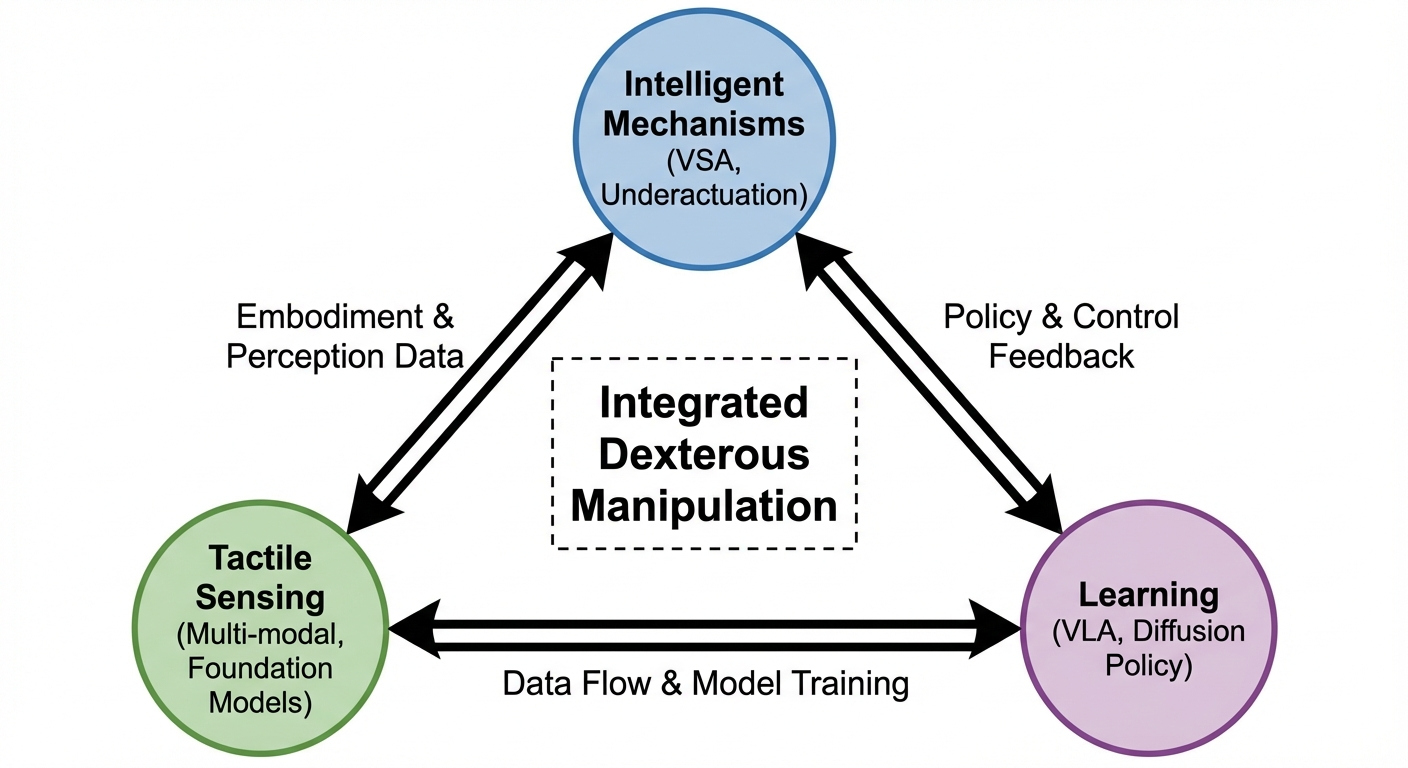
\includegraphics[width=\columnwidth]{../assets/figures/ch13/fig_13_4_triangle_integration_academic.png}
\caption{The proposed mechanism--tactile--learning triangle: intelligent mechanisms physically guarantee continuous contact, tactile sensors recognize the contact state, and learned policies exploit this information. The synergy among the three axes reduces the burden on each individual component and improves overall system robustness.}
\label{fig:triangle}
\end{figure}

\subsection{The Mechanism--Tactile--Learning Triangle}

We propose a unifying research direction that synthesizes the central insights of this survey:

\begin{itemize}
    \item \textbf{Mechanism axis} (Physical Intelligence): Intelligent mechanisms---underactuation, VSA, active surfaces, and their temporal integration---\emph{physically guarantee} continuous contact during manipulation (Section~\ref{sec:hands}). This improves state stability, simplifies the control problem, and reduces the frequency of destabilizing contact state transitions.

    \item \textbf{Tactile axis} (Sensing): Tactile sensors recognize the contact state during mechanism-induced continuous contact (Section~\ref{sec:sensors}), providing precise force measurement, slip detection, and material property estimation that enable closed-loop force control.

    \item \textbf{Learning axis} (Policy): VLA/Diffusion policies exploit the stable, information-rich tactile feedback from continuous contact states (Sections~\ref{sec:learning}--\ref{sec:vla}), achieving higher sample efficiency and better generalization than policies operating under the uncertainty of intermittent contact.
\end{itemize}

The key proposition is that \emph{when mechanism physically guarantees continuous contact, tactile recognizes the contact state, and learning exploits this information, the burden on each individual axis is reduced and the overall system robustness improves superlinearly}. The mechanism axis reduces the sensing challenge (stable contact $\to$ cleaner signals); the tactile axis reduces the learning challenge (rich feedback $\to$ fewer samples needed); and the learning axis enables the mechanism to be deployed in diverse, unstructured scenarios that pure mechanism design cannot anticipate.

This triangle connects the ``physical intelligence'' explored in Section~\ref{sec:mechanisms} with the ``software intelligence'' of Sections~\ref{sec:learning}--\ref{sec:vla}, offering a concrete path from current logistics-level industrial deployment to the manufacturing-grade dexterous manipulation that the field ultimately seeks. The key research question is: \emph{how should mechanism design, sensor placement, and policy architecture be jointly optimized to maximize the synergy among these three axes?}
